\documentclass{ugm-report}
\begin{document}
\begin{singlespace}
	\begin{center}
		\fontsize{14pt}{16pt}\selectfont
		Pengembangan Aplikasi Peranti Bergerak Lanjut:\\ Ide Tugas Akhir \\ Smart Lab Assistant\\
		\normalsize
		Nazmi Muhammad Abkary\\
		23/528925/PTK/15593
	\end{center}
\end{singlespace}

\section{Background}
Berkembangya teknologi edukasi dan laboratorium yang semakin banyak menggunakan perangkat digital dan peralatan yang memakan energy. Oleh karena itu, bermunculan beberapa masalah yang kemungkinan terjadi, diantaranya: penghamburan energi yang terjadi ketika peralatan lab menyala tanpa ada orang; management lampu, AC, dan peralatan lab yang manual; kurangnya data untuk optimalisasi penggunaan lab dan efisiensi energi; (kurangnya kemampuan untuk memonitor keadaan lab secara remote). \par
Aplikasi yang akan dibuat akan menggabungkan IoT (Internet Of Things) dengan sensor pada smartphone untuk memudahkan pengguna dalam memonitor keadaan dan  perangkat-perangkat di laboratorium. Aplikasi ini akan membantu pengguna dalam memantau keadaan laboratorium, mengontrol perangkat-perangkat yang ada di laboratorium, dan mengumpulkan data-data yang ada di laboratorium. Aplikasi ini juga akan membantu pengguna dalam mengoptimalkan penggunaan energi di laboratorium dengan mematikan perangkat-perangkat yang tidak digunakan.
\section{Aplikasi yang serupa}
Aplikasi serupa yang sudah ada di pasaran antara lain adalah Home Assistant. Home assistant merupakan project open-source yang mengintegrasikan banyak smart devices. Aplikasi serupa lainnya yaitu Smart Life, yaitu aplikasi closed-source yang juga mengintegrasikan berbagai smart devices. \par
Modifikasi yang akan dilakukan dalam pengembangan aplikasi smart lab ini adalah mengintegrasikan juga sensor-sensor yang ada pada smartphone. Sensor-sensor tersebut akan digunakan untuk mendukung smart devices yang ada pada laboratorium dalam pengolahan data.
\section{Sensor yang akan digunakan}
Sensor yang akan digunakan dalam aplikasi Smart Lab Assistant ini adalah sensor yang terdapat pada smartphone. Sensor-sensor tersebut antara lain:
\begin{itemize}
	\item Accelerometer atau Gyroscope\\
	      Sensor accelerometer atau gyroscope dapat digunakan dalam aplikasi Smart Lab untuk mendeteksi apakah pengguna sedang bergerak atau tidak.
	      Data tersebut dapat digunakan untuk mengetahui apabila pengguna laboratorium sedang berjalan, duduk, atau tidak bergerak yang dapat membantu dalam mengidentifikasi penggunaan laboratorium.
	\item Magnetometer atau Compass\\
	      Magentometer atau compass dapat digunakan untuk mengetahu orientasi atau arah gerakan pengguna.
	      Data tersebut dapat digunakan untuk membantu mendeteksi pengguna sedang berada di depan suatu perangkat atau tidak.
	\item Microphone\\
	      Sensor microphone dapat digunakan untuk mendeteksi suara-suara yang ada di sekitar pengguna. Sensor ini dapat digunakan untuk memonitor ambient sound level \textit{ambient sound level}. Data tersebut dapat digunakan untuk mengetahui tingkat aktivitas pada laboratorium. Microphone juga dapat digunakan untuk mendeteksi \textit{voice command} dari pengguna untuk mengontrol perangkat-perangkat yang ada di laboratorium.
	\item Light Sensor\\
	      Light Sensor dapat digunakan untuk mendeteksi tingkat cahaya pada laboratorium. Data tersebut dapat digunakan untuk mengkonfirmasi kondisi pencahayaan pada laboratorium dan mengetahui pola penggunaan laboratorium. Sensor ini dapat digunakan untuk mendeteksi apakah lampu menyala atau mati pada laboratorium.
	\item Camera\\
	      Camera digunakan untuk melakukan scanning QR code ketika pengguna melakukan checkin dan checkout pada laboratorium. Data tersebut, didukung oleh sensor lain, dapat digunakan untuk mengkonfirmasi keberadaan pengguna di laboratorium. Camera juga dapat digunakan untuk mendata perangkat yang akan digunakan oleh pengguna yang kemudian data tersebut dapat digunakan untuk monitoring penggunaan perangkat-perangkat yang ada di laboratorium.
	\item Wi-Fi dan Bluetooth\\
	      Wi-Fi dan Bluetooth dapat digunakan untuk mendeteksi keberadaan pengguna di laboratorium melalui Wi-Fi SSID (Service Set Identifier) atau Bluetooth beacon scanning. Data tersebut dapat digunakan untuk mengetahui apakah pengguna berada di sekitar laboratorium atau tidak. Data tersebut juga dapat digunakan untuk mengetahui pola penggunaan laboratorium berdasarkan lokasi pengguna dan siapa yang menggunakannya.
\end{itemize}
\section{Rencana pengolahan data}
Data akan diolah dengan menggunakan algoritma machine learning yang disimpan di Edge Computer pada laboratorium untuk mengidentifikasi pola-pola yang ada pada data sensor. Data yang dihasilkan dari sensor akan dikumpulkan dan dianalisis untuk mendapatkan informasi yang berguna bagi pengguna. 
Data yang telah diolah akan ditampilkan dalam sebuah dashboard. Dashboard ini akan menampilkan informasi mengenai pola penggunaan laboratorium, tingkat aktivitas pengguna, dan informasi lainnya. \par
Sensor-sensor pada smartphone akan aktif hanya setelah pengguna melakukan checkin melalui scan QR code. Contoh hasil pengolahan data sensor diantaranya adalah menghitung berapa perangkat yang telah melakukan checkin dan mengkonfirmasinya melalui Wi-Fi atau Bluetooth. Kemudian, sensor accelerometer dan gyroscope akan digunakan untuk menghitung tingkat aktivitas pada laboratorium, misalnya ketika jam praktikum dan data dari akselerometer dan gyroscope itu para pengguna tidak diam. Namun ketika ada jadual ujian pada laboratorium, sensor akselerometer tidak akan mendeteksi dan gyroscope akan mendeteksi seluruh pengguna memiliki orientasi yang sama. Sensor microphone akan digunakan untuk membantu memonitor keadaan laboratorium dari sisi ambient sound level yang akan di crosscheck dengan jumlah pengguna yang telah checkin. Light sensor akan digunakan untuk memonitor keadaan pencahayaan pada laboratorium yang akan di crosscheck dengan jumlah lampu yang menyala.

\begin{figure}[htbp]
	\centerline{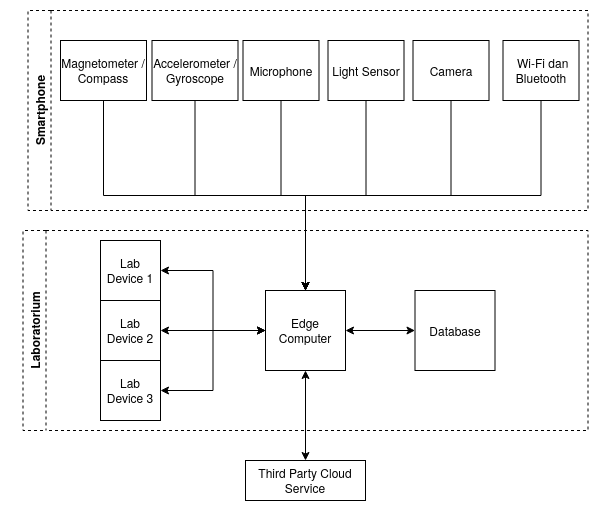
\includegraphics{image/fig1.png}}
	\caption{Architecture plan of the system.}
	\label{fig1}
\end{figure}

\url{https://github.com/Namury/mobile-development}
\end{document}